\begin{figure}[t]
\centering
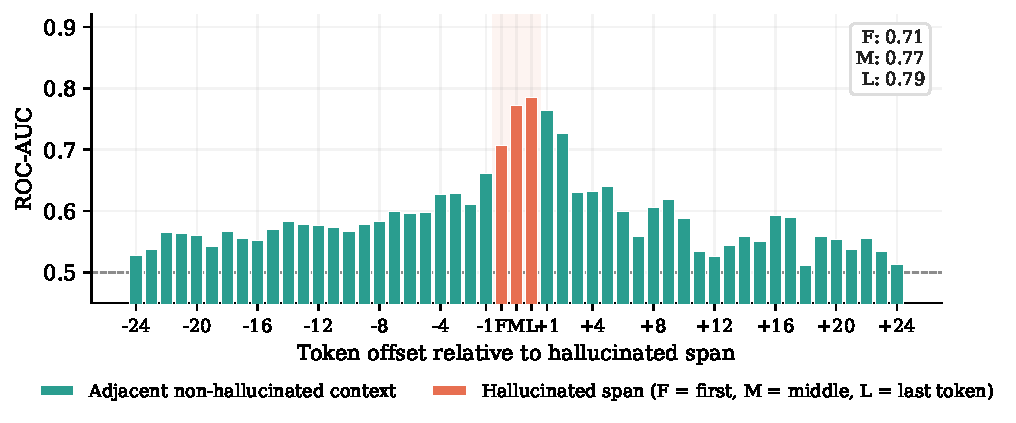
\includegraphics[width=0.95\linewidth]{figs/fig_signal_propagation.pdf}
\caption{Per-offset ROC-AUC of a linear probe (layer $L=1$ of the
$L=8$ pre-pooled hidden-state grid) measured on tokens at each offset
relative to a hallucinated span on RAGTruth (Llama-2-13b-chat). Teal
bars use the continuous non-hallucinated context adjacent to the span;
coral bars (F, M, L) are the first, middle, and last token of the
hallucinated span. Three regimes are visible: a pre-span ramp from
near-chance to AUC $\approx 0.66$ at offset $-1$ (anticipatory signal
one token ahead of the hallucination); a monotone in-span rise
$0.71 \to 0.79$; and post-span persistence that decays slowly back to
chance. The window-based localization of Section~\ref{sec:non_static}
exploits this neighborhood structure rather than treating tokens
independently.}
\label{fig:signal_propagation}
\end{figure}
